%!TEX root = synthese.tex
\newpage
\section{Design Pattern - Observer}

\subsection{Objectifs}

Les objectifs de l'incrément 2 sont les suivants :\\

\begin{itemize}
\item Synchroniser les historiques des terminaux;
\item Mettre à jour tous les terminaux lors de l'entrée d'une commande.\\
\end{itemize}

Afin de répondre à ces attentes, nous utiliserons le pattern Observateur. Nous avons décidé d’utiliser l’interface \emph{Observer} et la classe \emph{Observable} de Java. Ce pattern s’applique bien à cette situation car il permet la mise à jour de tous les objets « Observateurs » en fonction des objets «Observés ». Ici, la classe \emph{TerminalOS} sera l’observateur (Observer) et la classe \emph{User} sera observé (Observable).

\subsection{Implémentation}

\begin{figure}[!h]
\centering
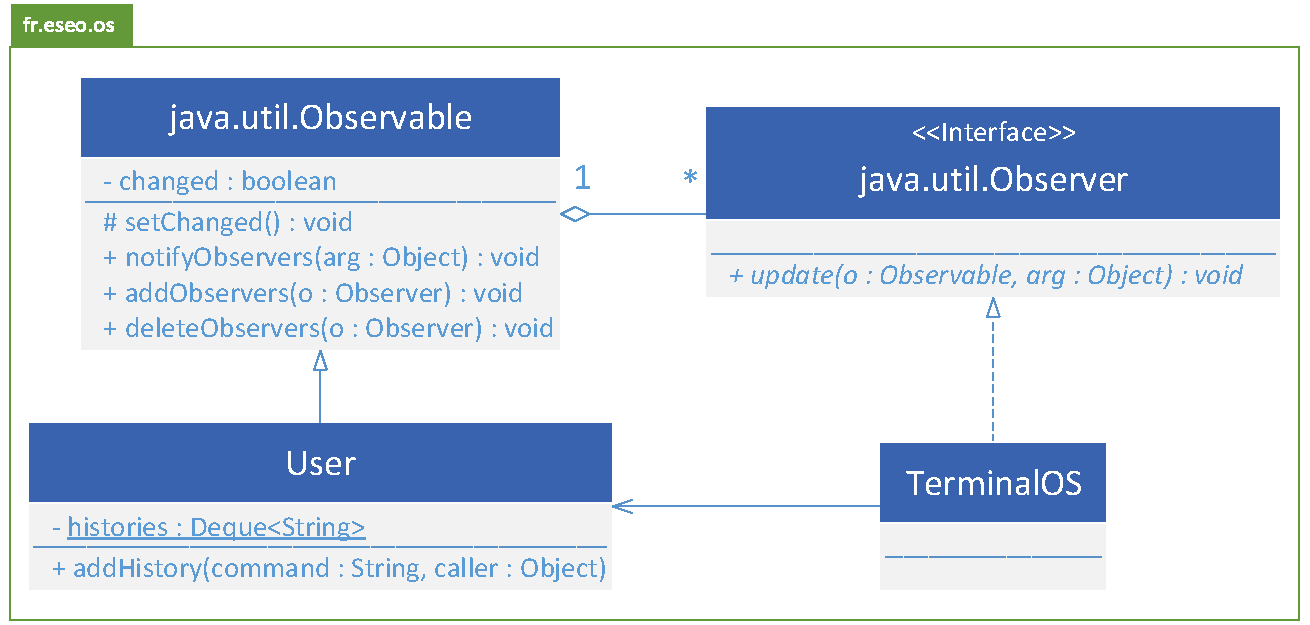
\includegraphics[width=\textwidth]{../uml/uml-observer}
\end{figure}

Pour commencer, nous avons implémenté l'interface \emph{java.util.Observer} dans la classe VirtualOS. 

\begin{lstlisting}
public class TerminalOS extends Terminal 
						implements Observer {...}
\end{lstlisting}

Ensuite, nous avons étendu la classe \emph{java.util.Observable} dans la classe \emph{User}. Cette classe a un historique (attribut \emph{histories}) collection de type \emph{Deque<String>}. Selon les spécifications d'Oracle, la collection \emph{Deque} est préférable dans notre cas (parcours de tous les éléments, ajout en queue d'un historique et récupération du dernier historique : LIFO\footnote{\emph{Last In First Out}}) plutôt que les collections \emph{List}, \emph{LinkedList} ou \emph{Stack}.

\begin{lstlisting}
public class User extends Observable {
    private Deque<String> histories;
    ...
}
\end{lstlisting}

Afin de gérer la synchronisation des historiques lors de l'ouverture d'un nouveau terminal, nous avons créé une méthode : \emph{fillHistory()}. Cette méthode parcours la liste des commandes du terminal courant et reproduit les entrées et sorties de l'utilisateur dans le nouveau terminal. Cette méthode est appelée dans le constructeur de \emph{TerminalOS}.

\begin{lstlisting}
private void fillHistory() {
	for(String historic : this.user.getHistories()){
		getCommandTA().append(historic);
	}
}
\end{lstlisting}

Ensuite, à chaque fois que l'utilisateur entre une commande (appelle la méthode \emph{handleCommand()}), on ajoute en queue la commande et son résultat. Cette fonctionnalité est implémentée dans la méthode \emph{addHistory()}.\\

Afin de gérer la synchronisation des terminaux, on utilise les méthodes de la classe \emph{Observable}. La méthode \emph{setChanged()} donne la possibilité de modifier les terminaux. La commande \emph{notifyObservers()}, fait appeler la méthode \emph{update()} de la classe \emph{TerminalOS} et donc modifie l'historie.

\begin{lstlisting}
public void addHistory(String command, Object caller){
    this.histories.add(command);
    this.setChanged();
    this.notifyObservers(caller);
}

@Override
public String handleCommand(String command){
	...
	user.addHistory(command + '\n' + result + '\n' + 
						user.getLogin() + PROMPT, this);
	return result;
}
\end{lstlisting}

Ensuite, on a \emph{override} la méthode \emph{update()} de \emph{TerminalOS} en ajoutant la commande et le résultat que nous voulions mettre à jour. On récupère seulement la dernière commande de l'historique.

\begin{lstlisting}
@Override
public void update(Observable o, Object caller) {
	if (caller != this) {
		tgetCommandTA().append(user.getHistories()
										.getLast());
	}
}
\end{lstlisting}

Enfin pour chaque nouveau terminal, il faut l'ajouter dans la liste des observer et remplir l'historique. On a modifié le contructeur comme suit :

\begin{lstlisting}
public TerminalOS(String login, String password){
	...
	this.fillHistory();
	this.user.addObserver(this);
}
\end{lstlisting}
